\section{Batteri}

Erfaringer fra tidligere studerenes bachelorprojekter viser, at batteriet til en Aeroquad quadrocopter belastes meget kraftigt (30-40 ampere). Derfor påkræves et batteri der momentvis kan klare et stort strømtræk. Ved valg af batteri stilles desuden krav til batteri type, spændingsniveau batteriet afgiver og batteriets samlede kapacitet.

Stort set alle batterier der bruges til RC projekter er LiPo batterier. Denne typer batteri er at foretrække fordi de har en mere flad afladningskurve. Dette betyder motorer mm. kan forsynes med den fornødne spænding længere - se afladningskurve \ref{fig:lipo_discharge}.

\begin{figure}[H]
\centering
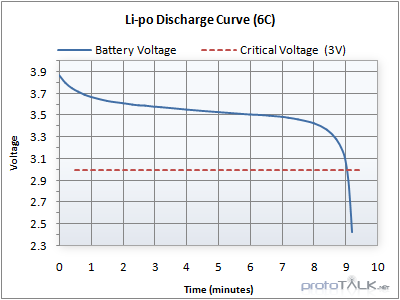
\includegraphics[width=0.7\textwidth]{Billeder/lipo_discharge_curve.png}
\caption{Afladning LiPo batteri}
\label{fig:lipo_discharge}
\end{figure}

De motorer dronen er udstyret med skal forsynes med 12V. Det betyder batteriet skal være 3 celler stort, ellers passer batteriets spændingsniveau ikke overens med den spænding der skal bruges til motorerne. For at spare penge og tid på gentagende gange at skulle købe nye batterier, prioriteres det også højt at batteriet der købes er genopladeligt. 

Stor kapacitet betyder at motorerne kan forsynes i længere tid, hvilket betyder at dronen kan blive i luften længere tid. Længere flyvetid giver bedre forudsætning til at udfører diverse test, særligt testflyvninger. Men et batteri med en stor kapacitet vejer generelt mere end et batteri med en mindre kapacitet. Så da dronen besidder begrænset løftekapacitet, sættes en naturlig grænse for batteriets kapacitet. Det gælder om at finde en god blanding af stor kapacitet og vægt. 
 
Valget af batteri faldt på et nano-tech 11.1 V batteri\footnote{http://www.hobbyking.com/hobbyking/store/\textunderscore\textunderscore 17247\textunderscore\textunderscore Turnigy\textunderscore \newline nano\textunderscore tech\textunderscore 4500mah\textunderscore 3S\textunderscore 35\textunderscore 70C\textunderscore Lipo\textunderscore Pack.html}. Dette batteri er 3 cellet, givet den rigtige udgangsspænding, tåler stor belastning og er genopladeligt. 

Foruden batteri, blev der også købt en tilhørende lader station\footnote{http://hobbyfly.com/opladere-tilbehoer-133/hobbyfly-hbc680-digital- \newline balance-lader-11-18v-80w-13248.html}.





